% !TEX TS-program = xelatex
% !TEX encoding = UTF-8 Unicode
% !Mode:: "TeX:UTF-8"

\documentclass{resume}
\usepackage{zh_CN-Adobefonts_external} % Simplified Chinese Support using external fonts (./fonts/zh_CN-Adobe/)
% \usepackage{NotoSansSC_external}
\usepackage{NotoSerifCJKsc_external}
% \usepackage{zh_CN-Adobefonts_internal} % Simplified Chinese Support using system fonts
\usepackage{linespacing_fix} % disable extra space before next section
\usepackage{cite}
\usepackage{graphicx}
\usepackage{tabu}
\usepackage{multirow}
\usepackage{progressbar}

\begin{document}
\pagenumbering{gobble} % suppress displaying page number

\Large{
  \begin{tabu}{ c l l }
   \multirow{5}{1in}{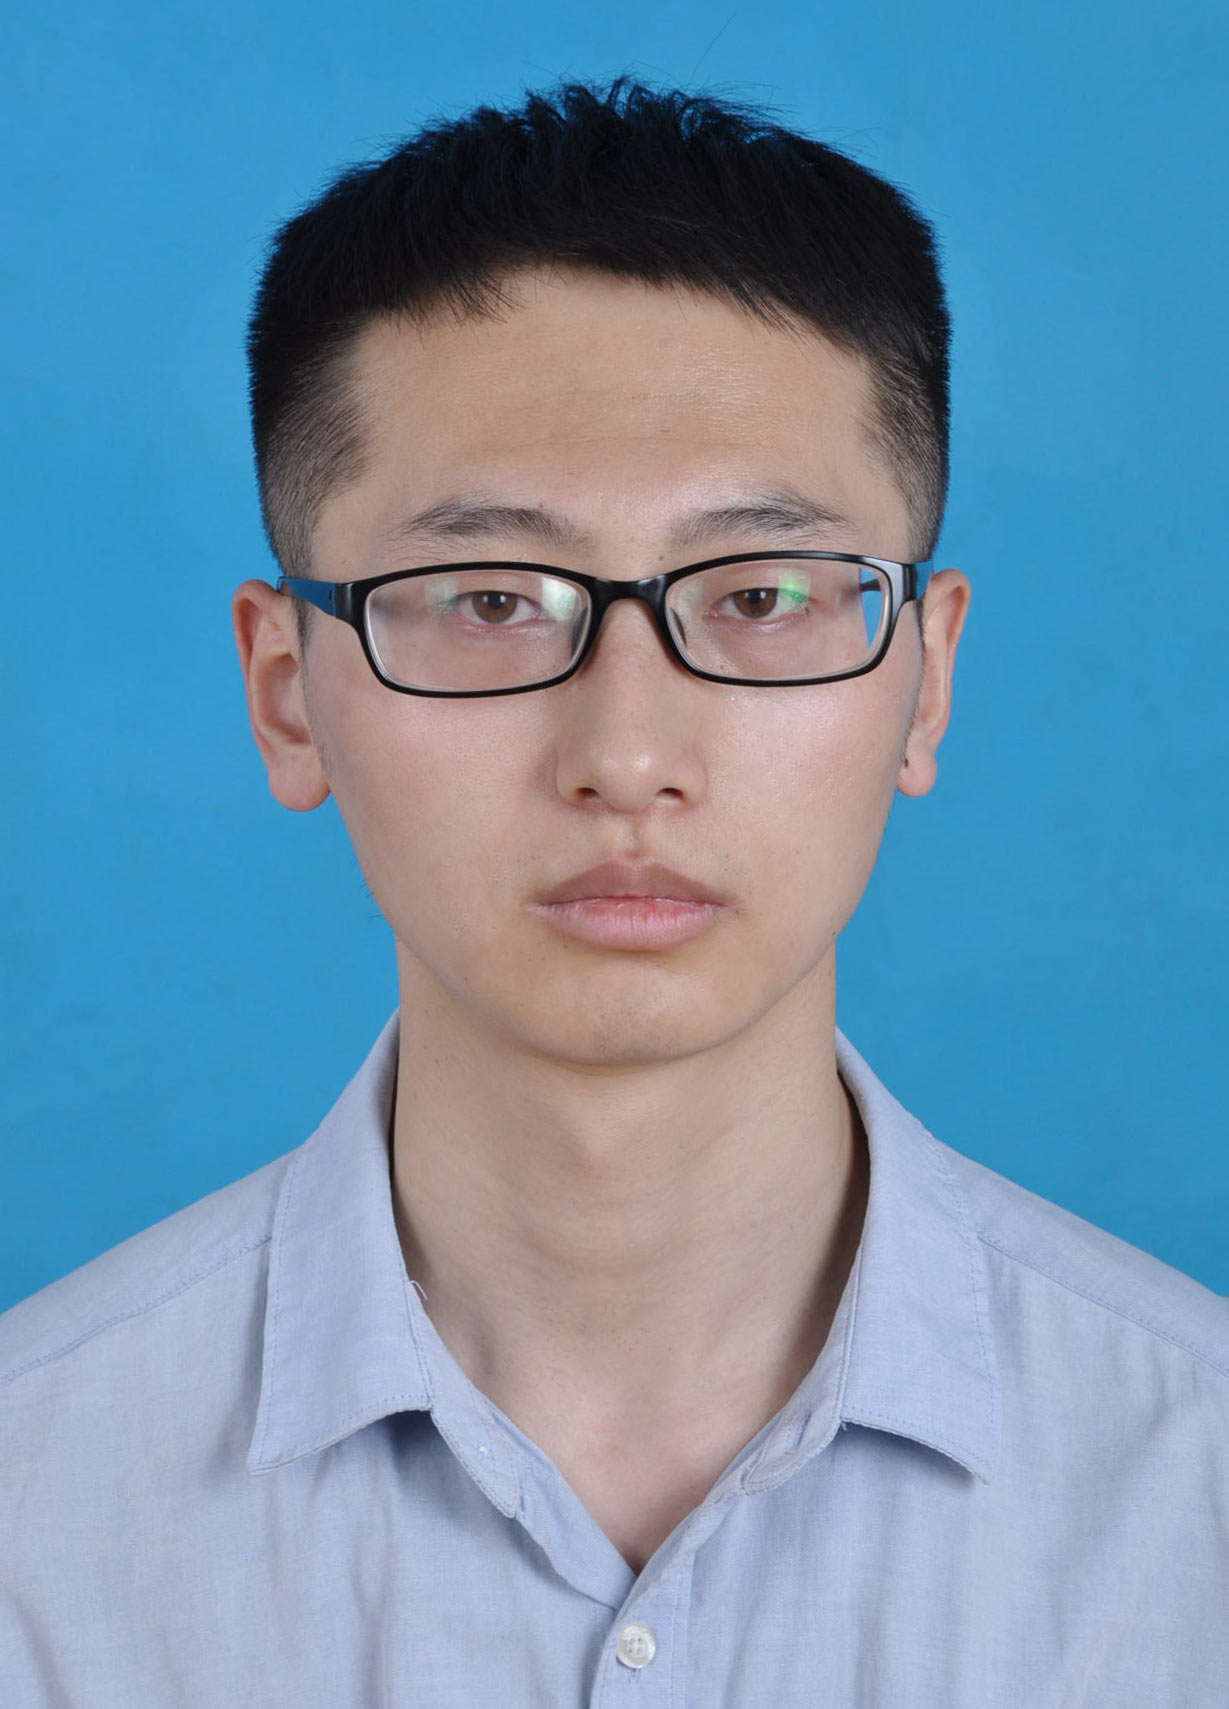
\includegraphics[width=0.88in]{avatar}} &
   \scshape{李高阳} &  \\
    & 性别:男 & 民族:汉 \\
    & 电话:(+86) 15682897374 & 生日:1995-09 \\
    & 邮箱:li.gaoyang@foxmail.com & 籍贯:甘肃宁县 \\
    & 地址:甘肃省兰州市天水南路222号 \ \ \ \ \ \ \ \ \ \ \ \ \ \ & 政治面貌:党员
  \end{tabu}
}

\section{教育经历}
% \textbf{兰州大学}
\datedsubsection{\textbf{兰州大学\ 硕博连读与中科院兰州近物所联合培养博士}}{2013 -- 2019}
\textit{专$\quad\ \ $业:理论物理}\\
\textit{研究方向:使用数值重整化群方法对杂质系统进行数值计算研究}\\
\textit{导$\quad\ \ $师:罗洪刚\ 教授(兰州大学) 李刚\ 研究员(近物所)}\\
\textit{副\hspace{7\ccwd}导\hspace{7\ccwd}师:房铁峰\ 副教授(兰州大学)}
\datedsubsection{\textbf{兰州大学\ 本科}}{2009 --  2013}
\textit{专业:物理学国家基地班}

\section{获奖情况}
\datedline{\textit{第一名}, xxx 比赛}{2013 年6 月}
\datedline{其他奖项}{2015}

\section{参与科研项目}
\begin{itemize}
\item 自然科学杰出青年基金(11325417):凝聚态理论与数值方法
\item 自然科学面上基金(11174115):少电子系统中电子关联的大尺度计算研究
\item 自然科学面上基金(11674139):量子杂质系统中的新奇量子态研究
\end{itemize}

\section{其他技能}
% increase linespacing [parsep=0.5ex]
\begin{itemize}[parsep=0.5ex]
\item 英语六级
\item 数值重整化群算法(NRG)
\item 擅长Fortran, C++, Shell, Python
\end{itemize}

\section{学术成果}
% increase linespacing [parsep=0.5ex]
\begin{itemize}[parsep=0.5ex]
  \item 使用数值重整化群方法研究了。我们发现了。
\end{itemize}

%% Reference
%\newpage
%\bibliographystyle{IEEETran}
%\bibliography{mycite}
\end{document}
